\chapter{Application of my Thesis}

To overcome the problems discussed in section \ref{current problem}, this thesis proposes a solution to automate the process of testing standalone modules
in Optislang. Since, the process is automated, the testing of modules needs to be done without the help of the \acrshort{gui}. To achieve this, a Python
\cite{python} framework is created to test the modules in an according manner. To use the framework in an automated manner, a \acrshort{ci} pipeline is created using GitHub Actions. The pipeline 
is triggered whenever a new commit is pushed to the repository. The pipeline runs the tests on the modules in a virtual machine and checks if the results are as expected. If the tests 
fail, the pipeline notifies the developer about the failure. The developer can then look into the issue and resolve it.

\section{DevOps}
Devops is the combination of a set of practices, tools which helps to automate and integrate the processes between software and organizations.

DevOps practices play a crucial role in the development of the automation process described in this thesis. By integrating \acrfull{ci} and \acrfull{cd} pipelines, we ensure that the testing of 
modules is efficient and reliable. This helps us to improve productivity and reduce human error. The DevOps approach allows for seamless collaboration between development and operations teams, 
ensuring that the testing framework and the modules it tests are consistently maintained and updated. This integration of DevOps practices not only enhances the quality of te software but also 
accelerates the development lifecycle, enabling faster delivery of new updates and features.
\begin{figure}[!h]
    \centering
    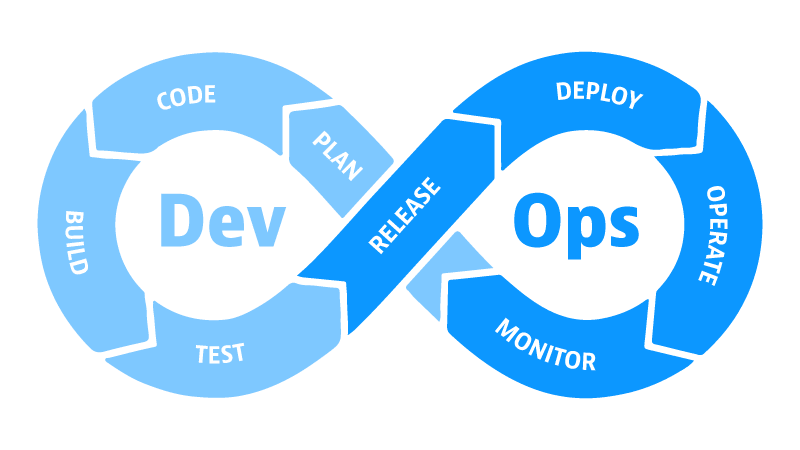
\includegraphics[width=0.7\textwidth]{Images/devops_loop.png}
    \caption{DevOps lifecycle}
    \label{devops_lifecycle}
\end{figure}

In summary, the application of DevOps in this thesis demonstrates how modern software engineering practices can be applied to automate and streamline the testing process, leading to more robust,
efficient and reliable software solutions.

\section{\acrfull{ci}}

\section{Code quality}